\section{Turno del jugador}

La mayor parte del juego es un bucle de turno del jugador y turno de la casa, para iniciar se pregunta qué cantidad de dinero quieres apostar, el dinero que se puede apostar tiene que ser igual o menor al dinero que se tiene. En tu primer turno el dinero será el depositado, luego cambiará dependiendo de tus victorias y pérdidas. Si tu dinero es igual a 0 puedes pedir un préstamo para obtener más dinero, pero esto generará una deuda que se te cobrará al inicio de cada turno.

Volviendo, luego de realizar tus apuestas tienes 3 opciones, la primera es duplicar tu apuesta si tu dinero es igual o mayor al doble de la apuesta realizada, la segunda opción es robar, con la cual obtienes una carta extra y,finalmente, está la opción de quedarte para finalizar tu turno.

Ahora se explicará de forma más detallada como funciona y las variables del turno:

\newpage

\subsection{Dinero y deuda}

El juego se desarrolla en base a apuestas y por ende dinero, el dinero inicial que tendras es el que se ingresara al inicio del juego, luego en base a este dinero y apuestas se puede aumentar o perder, el objetivo del jugador es obtener la mayor cantidad de dinero posible sin llegar a un limite, esto para que el jugador pueda jugar hasta el punto que quiera. Al ganar una apuesta duplicas el dinero apostado y en caso de perder se te restara el dinero apostado.

En caso que te quedes sin dinero puedes pedir un prestamo teniendo 2 variables, en la primera pierdes por tener mas de 21 puntos y en el segundo caso pierdes porque la casa te supera, la diferencia entre ambas es el aspecto visual, ya que, dependiendo del caso sera el esqueleto chistoso sin derechos de autor sera quien te preste el dinero.

En el primer caso de perder por pasarte de 21 puntos aparecerá el esqueleto Sens (no confundir con Sans):
\begin{figure}[h]
    \raggedright
    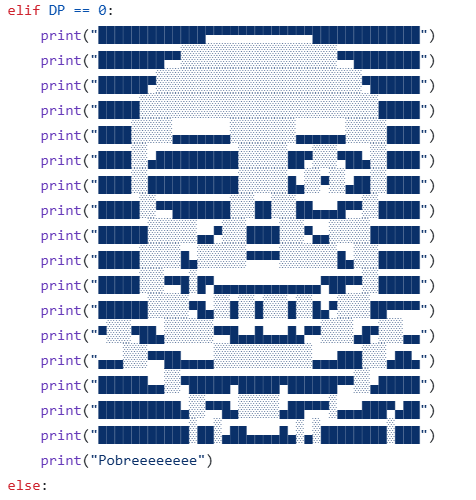
\includegraphics[width=0.5\linewidth]{Imagenes/sens.PNG}
    \label{fig:}
\end{figure}

\newpage

En el segundo caso es el perder porque la casa te supera en puntaje sin pasarse del limite, en este caso aparecerá Luigi el esqueleto:
\begin{figure}[h]
    \raggedright
    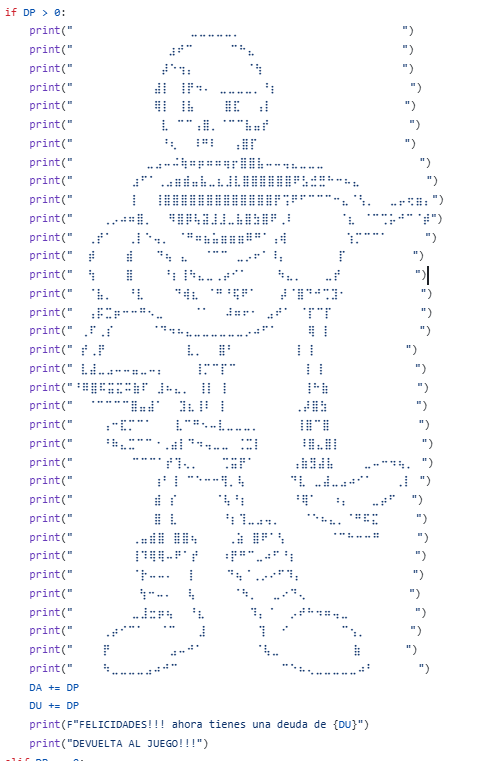
\includegraphics[width=0.7\linewidth]{Imagenes/luigi.PNG}
    \label{fig:}
\end{figure}

En ambos casos se te preguntara si te quieres endeudar, en caso de decir que no el juego termina, y en caso de decir que si se te preguntara la  cantidad, en caso de poner 0 el juego también terminara y cualquier otra cantidad sera aceptada pasándose a tu dinero y aumentando esa cantidad tu deuda.

La deuda se va pagando con tus turnos, cuando tu dinero es igual o mayor a la mitad de la deuda se te restara esta mitad reduciendo tu deuda hasta llegar a 0.

\newpage

\subsection{BlackJack}

Existe la posibilidad de obtener un \textbf{"BlackJack"} el cual es una victoria instantánea, esta se obtiene al obtener una \textbf{A} (tradicionalmente aunque puede ser remplazado con un \textbf{JOKER}) y una letra de valor 10 (\textbf{JOKER, J, Q} y \textbf{K}). El \textit{Blackjack} puede ser del jugador o de la casa.

\begin{figure}[h]
    \centering
    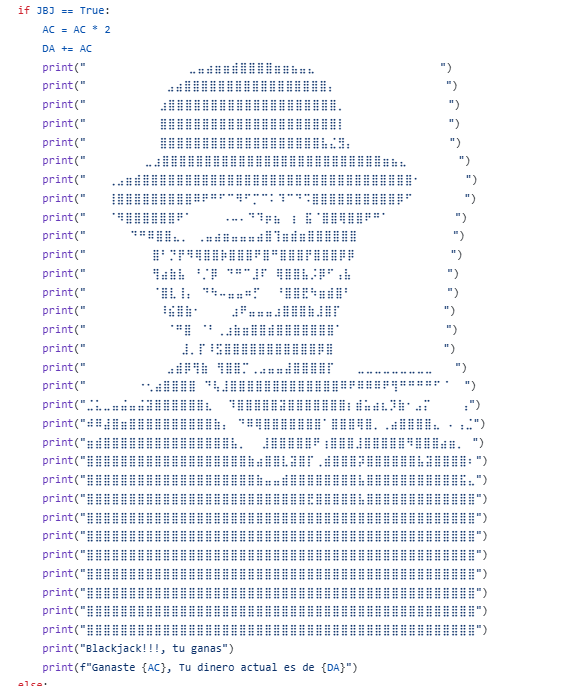
\includegraphics[width=0.4\linewidth]{Imagenes/BlackJack J.PNG}
    \hspace{0,1cm}
    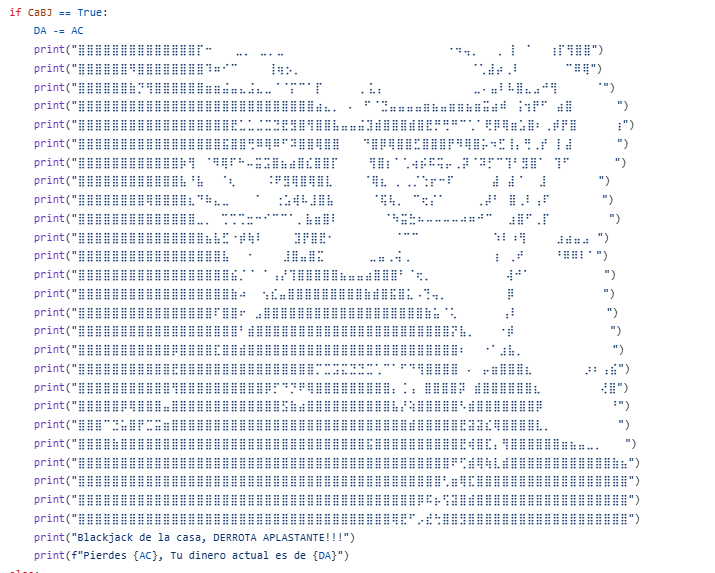
\includegraphics[width=0.5\linewidth]{Imagenes/BlackJack C.PNG}
\end{figure}

\subsection{Robo}

El sistema de robo se hace mediante el "\textit{import random}" Y La función "\textit{random.randint}". La función puede retornar un numero entre 0 y 13, dependiendo de este numero se daba el valor de la carta, en la mayoría de casos era igual al numero a excepción de 0, 1, 11, 12 y 13 que equivales a \textbf{JOKER}, \textbf{A}, \textbf{J}, \textbf{Q} y \textbf{K} respectivamente.

La opción de robo se repetirá en bucle hasta que: tu puntaje sea mayor a 21 perdiendo o que el jugador eligiera la opción de quedarse.

\subsection{Quedarse}

Puedes quedarte para finalizar el bucle y pasar al turno de la casa.

\newpage